\documentclass{tufte-handout}

%\geometry{showframe}% for debugging purposes -- displays the margins

\usepackage{amsmath}

% Set up the images/graphics package
\usepackage{graphicx}
\setkeys{Gin}{width=\linewidth,totalheight=\textheight,keepaspectratio}
\graphicspath{{graphics/}}

\title{A Lagrangian Perspective on the Lifecycle and Cloud Radiative Effect of Deep Convective Clouds Over Africa}
\author[William Jones]{William Jones, Martin Stengel, Philip Stier}
\date{Gordon Research Conference Radiation \& Climate 2023}  % if the \date{} command is left out, the current date will be used

% The following package makes prettier tables.  We're all about the bling!
\usepackage{booktabs}

% The units package provides nice, non-stacked fractions and better spacing
% for units.
\usepackage{units}

% The fancyvrb package lets us customize the formatting of verbatim
% environments.  We use a slightly smaller font.
\usepackage{fancyvrb}
\fvset{fontsize=\normalsize}

% Small sections of multiple columns
\usepackage{multicol}

% Provides paragraphs of dummy text
\usepackage{lipsum}

% These commands are used to pretty-print LaTeX commands
\newcommand{\doccmd}[1]{\texttt{\textbackslash#1}}% command name -- adds backslash automatically
\newcommand{\docopt}[1]{\ensuremath{\langle}\textrm{\textit{#1}}\ensuremath{\rangle}}% optional command argument
\newcommand{\docarg}[1]{\textrm{\textit{#1}}}% (required) command argument
\newenvironment{docspec}{\begin{quote}\noindent}{\end{quote}}% command specification environment
\newcommand{\docenv}[1]{\textsf{#1}}% environment name
\newcommand{\docpkg}[1]{\texttt{#1}}% package name
\newcommand{\doccls}[1]{\texttt{#1}}% document class name
\newcommand{\docclsopt}[1]{\texttt{#1}}% document class option name

\begin{document}

% \begin{fullwidth}
\maketitle% this prints the handout title, author, and date
% \end{fullwidth}

\begin{abstract}
\noindent Contact email: william.jones@physics.ox.ac.uk
\end{abstract}

%\printclassoptions

% \subsection{Introduction}

%\newthought{The anvil clouds of tropical deep convection} have large shortwave~(SW) and longwave~(LW) cloud radiative effect~(CRE), with both averaging over 100\,Wm$^{-2}$.
The anvil clouds of tropical deep convection have large shortwave~(SW) and longwave~(LW) cloud radiative effect~(CRE), with both averaging over 100\,Wm$^{-2}$.
Despite this, the net CRE of tropical anvil clouds is zero as these two components cancel each other out\cite[-3.5\baselineskip]{hartmann_balanced_2017}.
A number of hypotheses (e.g.\ fixed anvil temperature\cite{hartmann_important_2002}, iris hypothesis\cite{lindzen_does_2001}) have proposed mechanisms through which the CRE balance may respond to a changing climate.
These hypotheses do not however consider how the the CRE of anvil clouds are impacted by the diurnal cycle of deep convection.
In this study, we aim to better understand the relationship between the diurnal cycle and lifetime of convection and the anvil cloud CRE using geostationary satellite observations.


\subsection{Method}\label{sec:method}

\begin{marginfigure}%
  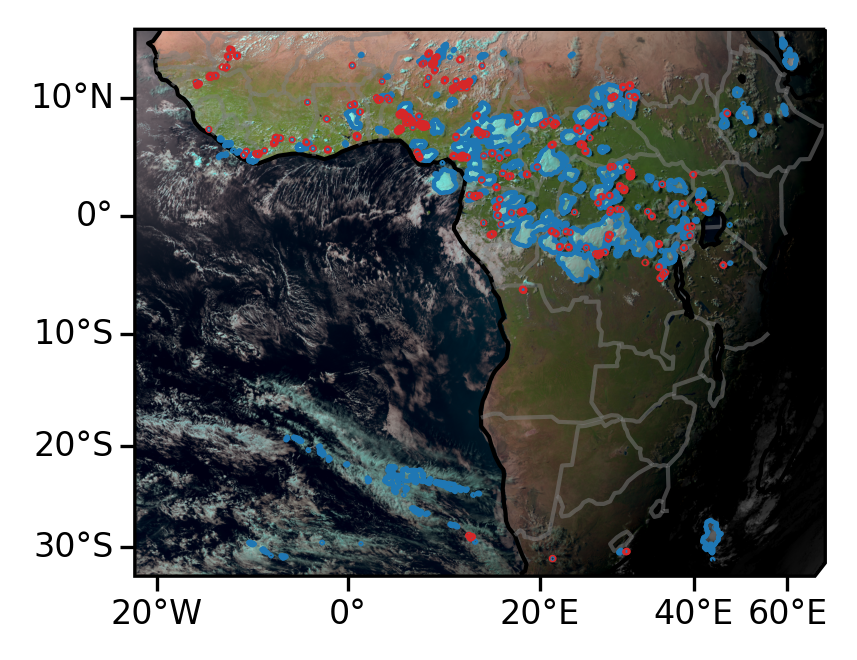
\includegraphics[width=\linewidth]{figures/handout_fig1.png}
  \caption{Detected cores (red) and anvils (blue) in a SEVIRI image}
  \label{fig:marginfig}
\end{marginfigure}

Geostationary satellite instruments provide a unique view of deep convection, with a combination of high spatial and temporal resolution over large domains and long time series that are not available from other sources.

We explicitly calculate the CRE for four months of Meteosat SEVIRI\cite[0.5\baselineskip]{aminou_characteristics_1997} data using a broadband radiative flux model.
The SW and LW CRE are validated against monthly CERES observations, and the calculated bias is removed from all subsequent CRE values.

\begin{marginfigure}%[0.5\baselineskip]%
  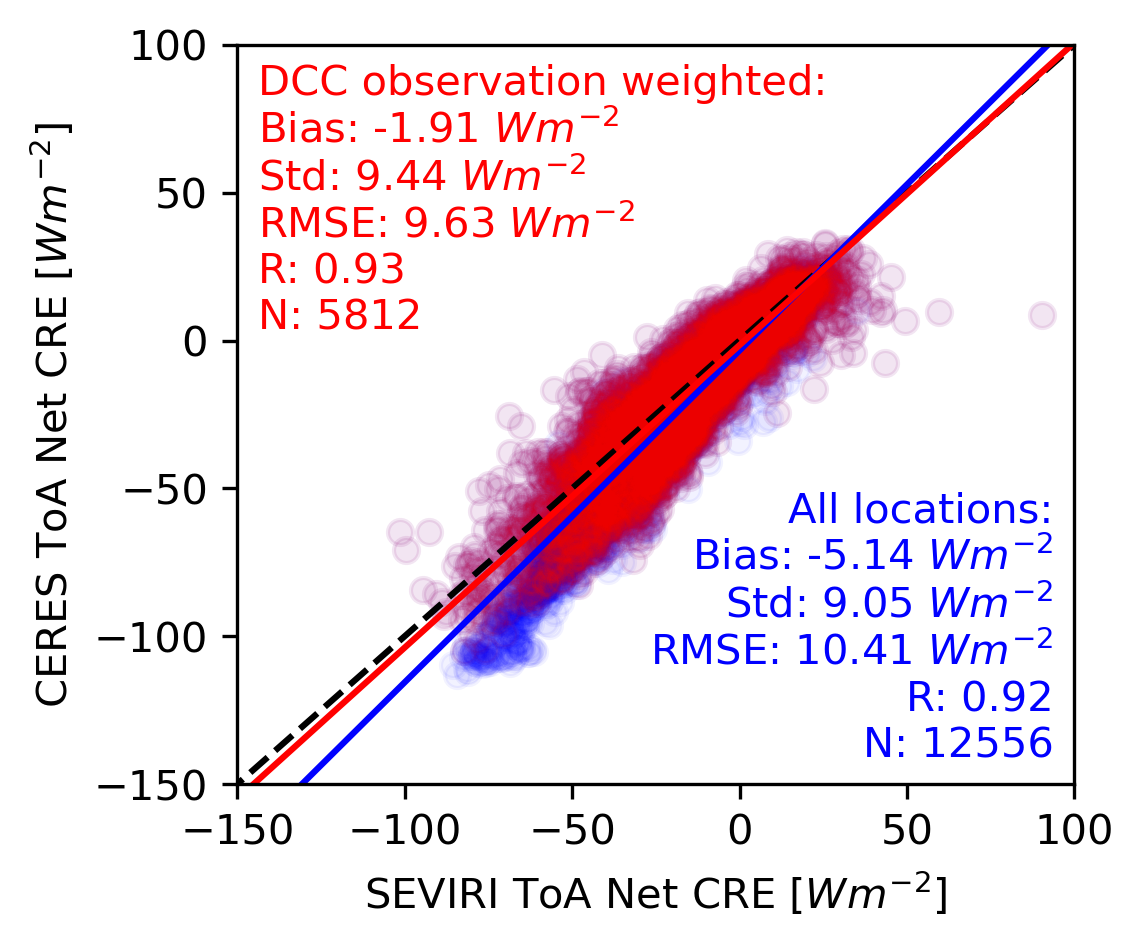
\includegraphics[width=\linewidth]{figures/handout_fig2.png}
  \caption{Comparison of CRE observations from CERES and SEVIRI retrieval, for all locations (blue) and weighted by locations where DCCs are observed (red)}
  \label{fig:marginfig}
\end{marginfigure}

A novel, semi-Lagrangian algorithm is used to detect and track deep convective clouds~(DCCs).
We first use an optical flow method to estimate the cloud motion vectors in the sequence of observations.
Growing convective cores are then detected where we observe rapid cooling rates in brightness temperature, indicating vertical ascent.
The associated anvil clouds are then detected using the water vapour difference field, and continue to be tracked even after the associate core is no longer detected.
By accounting for the cloud motion, we are able to track DCCs across a range of scales from isolated convection to large, long-lived mesoscale convective systems~(MCSs).

CRE, along with other properties such as area and cloud-top temperature are then calculated along the lifecycle of each DCC, allowing their properties to be investigated.

\subsection{Lifecycle}



The DCCs tracked in this study cover a range of lifecycles, from short-lived, isolated systems to multi-core MCSs.
The majority of convection observed in this study occurs over land, with a peak of convective activity in the late afternoon and early evening.
% The proportion of the anvil cloud which exists at nighttime depends on both the time of initiation of the DCC and the lifetime.
Isolated DCCs occurring earlier in the day tend to have anvils which occur entirely in daylight hours, with those initiating later dissipating during the twilight and nighttime.
However, longer-lived DCCs tend to have more of the anvil cloud lifetime at night.
MCSs existing for multiple days tend to smooth out this diurnal cycle, and so the time of initiation has a smaller effect on their properties.

\begin{marginfigure}[-15\baselineskip]%
  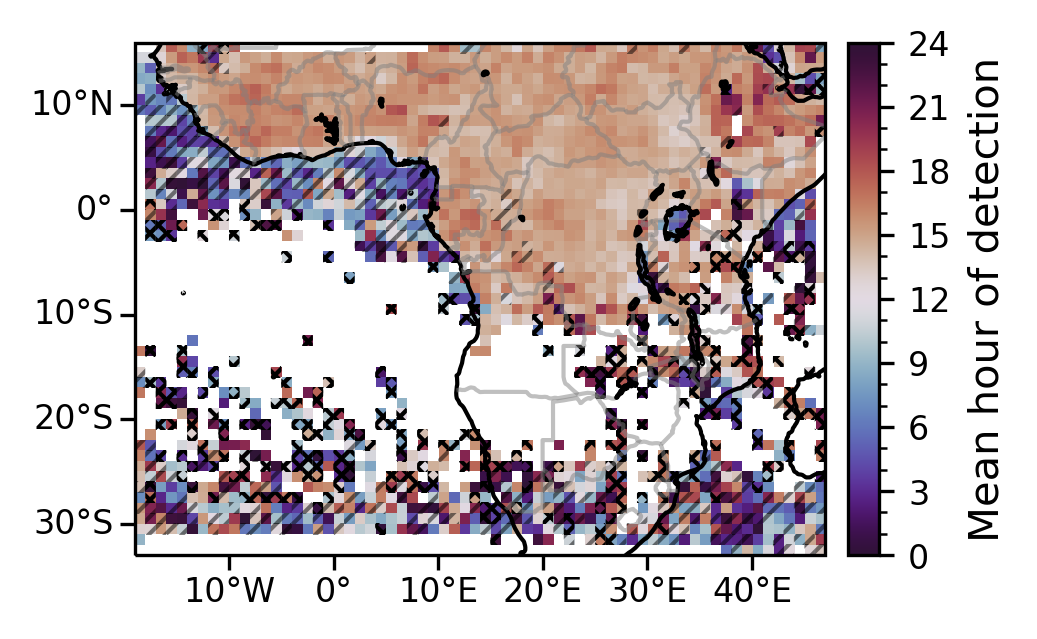
\includegraphics[width=\linewidth]{figures/handout_fig3.png}
  \caption{The average time of detection in each 1\texttimes 1\textdegree grid box. Locations with larger variance are shown hatched}
  \label{fig:marginfig}
\end{marginfigure}

\begin{marginfigure}%
  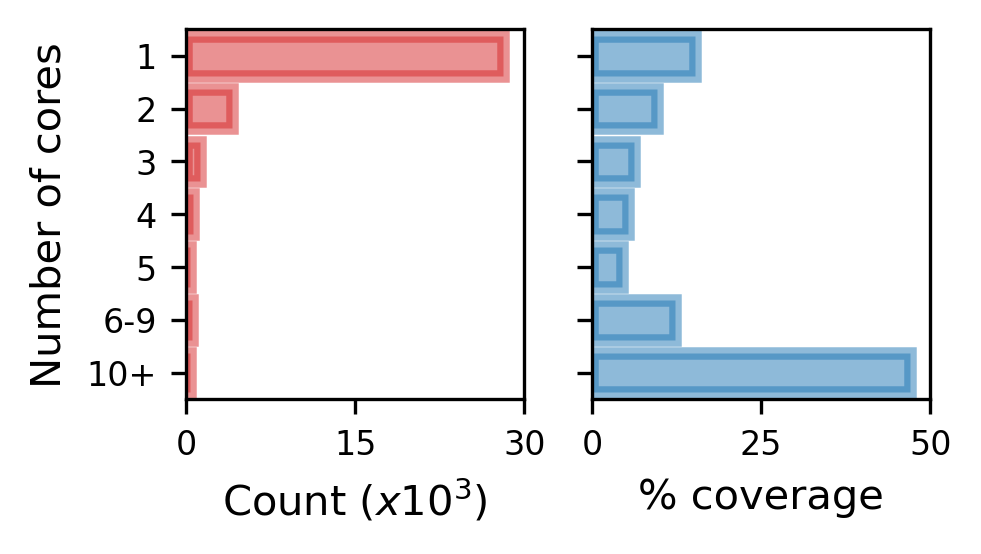
\includegraphics[width=0.95\linewidth]{figures/handout_coverage_figure.png}
  \caption{The count of DCCs with differing number of cores (red) and their percentage contribution to total anvil coverage (blue).}
  \label{fig:marginfig}
\end{marginfigure}

The majority of DCCs detected have a single core, however we also detect a large number of multi-core systems.
There is a strong tendency for anvils with multiple cores to have longer lifetimes, larger areas and colder cloud-top temperatures.
Despite only making up a small proportion of the overall number of systems, DCCs with 10 or more cores are responsible for over 50\% of the total anvil coverage.


\subsection{Cloud Radiative Effect}

\begin{marginfigure}[1\baselineskip]%
  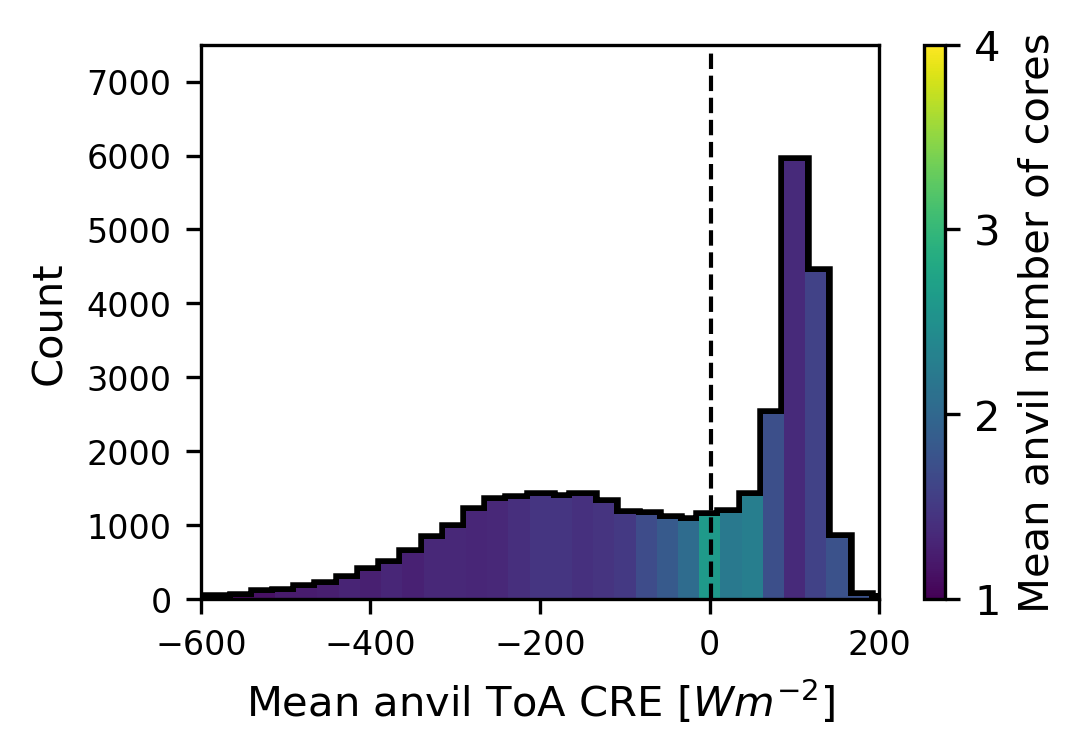
\includegraphics[width=\linewidth]{figures/handout_fig4.png}
  \caption{The distribution of anvil CRE. The colour scale shows the average number of cores for anvils in each bar.}
  \label{fig:marginfig}
\end{marginfigure}

The CRE of individual DCCs is strongly influenced by the diurnal cycle of the SW CRE, with DCCs occurring during the daytime having a strong cooling effect, and those occurring at night having a warming effect.
As a result, the distribution of DCC CRE has a bimodal shape, with the two peaks corresponding to those DCCs which occur during the day- and nighttime.
Very few individual DCCs have net CRE near zero, and these tend to be larger, multi-core systems which exist for more of the diurnal cycle.

\begin{marginfigure}[1\baselineskip]%
  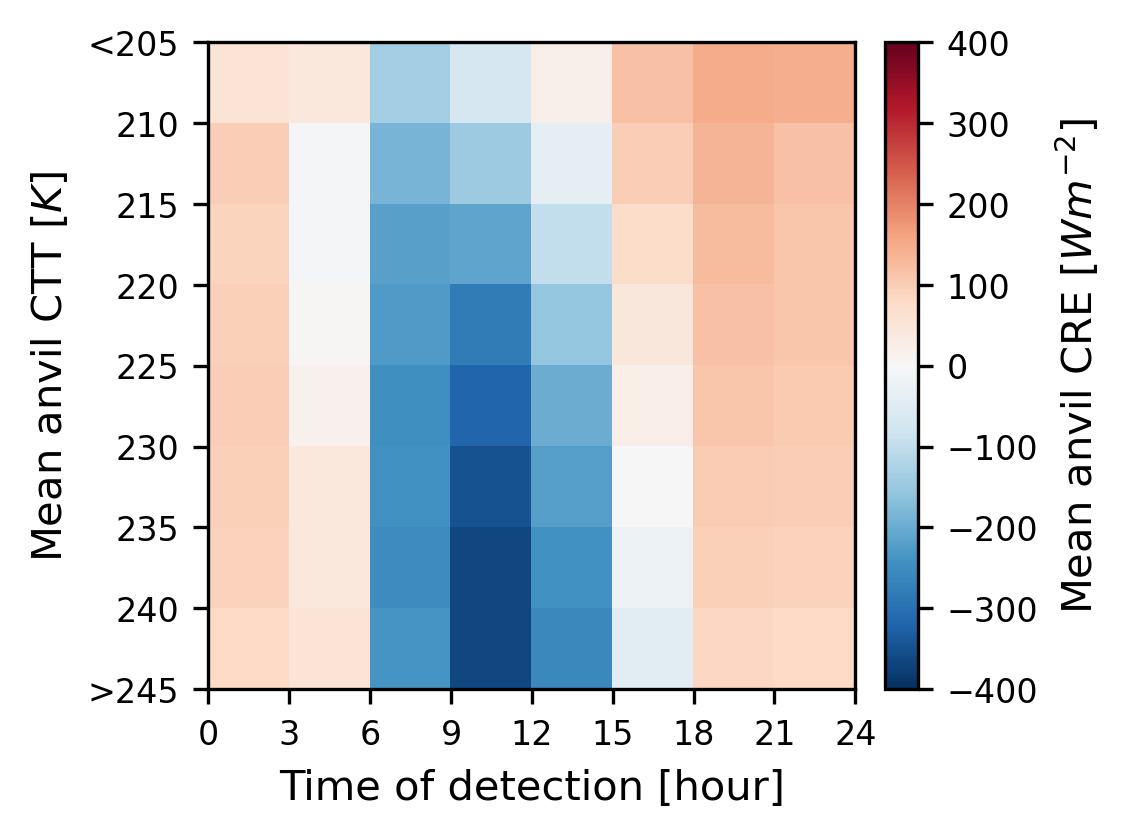
\includegraphics[width=\linewidth]{figures/handout_fig5.png}
  \caption{The average CRE of anvils binned by time of initiation and CTT. Anvils with warmer CTT---which tend to be isolated, short-lived systems---show more variation across the diurnal cycle.}
  \label{fig:marginfig}
\end{marginfigure}

Despite this, the overall average anvil CRE (accounting for anvil area and lifetime), is still zero.
While larger MCSs have a large contribution to this due to their large area, isolated DCCs have a disproportionately large influence due to their strong cooling or heating effects.
As a result, isolated DCCs are more important for the overall CRE balance than their proportion of anvil area would suggest.

\subsection{Summary}

Time of initiation and lifetime has an important effect on the CRE of individual DCCs---in particular for isolated DCCs---despite the overall balance being zero.
Understanding how the lifecycle of DCCs changes in response to a changing climate is vital to understanding DCC CRE feedbacks.
Changes in time of initiation, convective strength, organisation and anvil cloud dissipation may all play a role in future changes in anvil CRE.


\nobibliography{references}
\bibliographystyle{apalike}



\end{document}
